% Intended LaTeX compiler: pdflatex
\documentclass[10pt,a4paper,UTF8]{article}
\usepackage{zclorg}
\usepackage{tikztheorem}
\author{zcl.space}
\date{}
\title{Composition and Inverse}
\hypersetup{
 pdfauthor={zcl.space},
 pdftitle={Composition and Inverse},
 pdfkeywords={PMA},
 pdfsubject={},
 pdfcreator={Emacs 25.0.50.1 (Org mode 9.1.2)},
 pdflang={English}}
\begin{document}

\maketitle
\tableofcontents
\titlepic{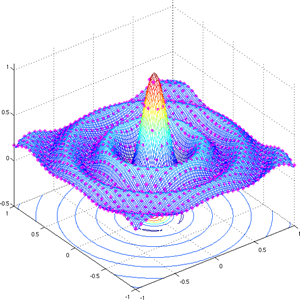
\includegraphics[scale=0.25]{../../img/sinc.PNG}}
 If \(f:X\to Y\) and \(g:Y\to Z\), then the \textbf{composition}
of \(f\) and \(g\) is the map \(g\circ f:X\to Z\) defined by
$$
    (g\circ f)(x)=g(f(x))
$$
for \(x\in X\).
For any set \(X\) the \textbf{identity map}  of \(X\)
is the map \(\mathrm{id}_X:X\to X\) defined by
$$
  \mathbb{I}_X(x)=x
$$
for \(x\in X\).  Clearly
$$
    \mathbb{I}_Y\circ f = f \mbox{ and } f\circ \mathbb{I}_X=f
$$
for \(f:X\to Y\).

A map \(g:Y\to X\) is said to be
a \textbf{left inverse}
for the map \(f:X\to Y\) iff \(g\circ f= \mathbb{I}_X\), i.e.
iff \(g(f(x))=x\) for all \(x\in X\).
A map \(g:Y\to X\) is said to be a \textbf{right inverse}
for the map \(f:X\to Y\) iff \(f\circ g=\mathbb{I}_Y\), i.e.
iff \(f(g(y))=y\) for all \(y\in Y\).
A map \(g:Y\to X\) is said to be  a (two sided) \textbf{inverse}
to the map \(f:X\to Y\) iff it is both
a left inverse and a right inverse to \(f\).
 If \(g\) is a left inverse to \(f\) and \(g'\) is a right inverse
to \(f\) then \(g=g'\).
(Proof: \(g=g\circ \mathbb{I}_X=g\circ f\circ g'=\mathbb{I}_Y\circ g'=g'\).)
In this case there is a unique inverse and it is denoted \(f^{-1}\).
So if \(f:X\to Y\) has an inverse \(f^{-1}:Y\to X\), then
$$
           y=f(x)\iff x=f^{-1}(y)
$$
for \(x\in X\) and \(y\in Y\).

 A map \(f:X\to Y\) is said to be \textbf{injective}
iff
$$
  \forall x_1,x_2\in X\;[f(x_1)=f(x_2)\implies x_1=x_2]
$$
and it is said to be \textbf{surjective}  iff \(Y=f(X)\), i.e.
$$
\forall y\in Y\;\exists x\in X\; y=f(x).
$$
A map is \textbf{bijective}  iff it is both injective and surjective.
Thus

\begin{enumerate}
\item A map is injective if and only if it has a left inverse;
\item A map is surjective if and only if it has a right inverse;
\item A map is bijective  if and only if it has a (two-sided)  inverse.
\end{enumerate}

a map is surjective if and only if its range equals its target.

 Both Lang and Morgan use the more modern terms injective, surjective, bijective,
but Buck and Rudin use the older terminology
\textbf{one-one}  instead of injective,
\textbf{onto}  instead of \textbf{surjective}, and
\textbf{one-one onto}  instead of bijective.
The older terminology is used in teaching calculus.

The 'only if' part of item\textasciitilde{}(2) is called the \textbf{Axiom of Choice} .
It was once controversial because one can imagine a situation where
one can prove that a map \(f\) is surjective but where one cannot give
an explicit formula for a right inverse.


The assertions (1-3)  are false if continuity (defined later) is required:
There is a continuous bijective  map whose inverse is not continuous
(and hence continuous injective map which does not have a continuous left inverse,
and a continuous surjective map which does not have a continuous right inverse).
Let \(S:=\{(x,y)\in\mathbb{R}^2: x^2+y^2=1\}\) denote the unit circle in \(\mathbb{R}^2\)
and define \(f:[0,2\pi)\to S\) by \(f(\theta)=(\cos\theta,\sin\theta)\).
Then \(f\) bijective and continuous but \(f^{-1}\) is not continuous.
We will see that the inverse if a
continuous  bijective map is continuous if its domain is compact (defined later),
but \([0,2\pi)\) is not compact.


Consider the four maps
$$
f_1:\mathbb{R}\to\mathbb{R},\quad f_2:[0,\infty)\to\mathbb{R}, \quad f_3:\mathbb{R}\to[0,\infty), \quad f_4:[0,\infty)\to [0,\infty)
$$
defined by \(f_i(x)=x^2\). Then \(f_1\) is not injective and not bijective, \(f_2\) is injective but not surjective,
\(f_3\) is surjective but not injective, and \(f_4\) is bijective. Any map \(g_2:\mathbb{R}\to[0,\infty)\)
such that \(g_2(y)=\sqrt{y}\) for \(y\ge 0\) is a left inverse to \(f_2\), and any map \(g_3:[0,\infty)\to\mathbb{R}\)
such that \(g_3(y)=\pm\sqrt{y}\) (the \(\pm\) can depend on \(y\)) is a right inverse to \(f_3\)
The inverse map to \(f_4\) is \(f_4^{-1}(y)=\sqrt{y}\).
\end{document}
